\chapter*{Introducere} 
\addcontentsline{toc}{chapter}{Introducere}

\section*{Context}
\paragraph{}
Știință și tehnologie.
Acest duo se regăsește la orice pas al secolului XXI și interacționăm cu el zilnic, mai mult sau mai puțin, prin intermediul telefoanelor, al televizoarelor și al calculatoarelor care sunt la dispoziția noastră și prin intermediul multor altor dispozitive.
Într-o formă sau alta, dispozitivele de acest fel (\emph{împreună} cu mulțimea de aplicații software pe care le rulează) fac lumea mai \emph{accesibilă} pentru utilizatorii lor – de pildă, să verificăm vremea zilei de mâine pe un laptop sau să ne bazăm pe comenzile online în timpul unei pandemii.
Astfel de exemple ne arată cum tehnologia modelează felul în care ne desfășurăm activitățile zilnice și ``scurtăturile'' pe care le putem lua pentru a îndeplini anumite sarcini – desigur, în anumite cazuri, cu niște costuri aferente.

\paragraph{}
În paragraful de mai sus este accentuat termenul ``accesibil'' care, prin definiție\footnote{Definiție preluată din DEX 2009}, înseamnă ceva ``care este la îndemâna cuiva; care poate fi ușor procurat''.
Am văzut cum lumea poate fi ``mai la îndemâna cuiva'' – dar cum facem ca tehnologia să fie, la rândul ei, accesibilă?
Cum ar putea, spre exemplu, o persoană paralizată să folosească un laptop?

\paragraph{}
După o analiză retrospectivă putem constata că oamenii au lucrat dintotdeauna la modalități (de exemplu la dezvoltarea de software) pentru a face tehnologia mai accesibilă oamenilor.
Un exemplu ar fi ``Cititorul de ecran'' (în engleză ``Screen reader''), care este incorporat în majoritatea smartphone-urilor recent lansate, sau asistentul inteligent precum Siri, Bixby sau Google Assistant.
Acestea pot permite persoanelor oarbe să interpreteze conținutul unui ecran digital sau unei persoane imobilizate să asculte muzică, să afle noutăți ș.a.m.d.
Acest tip de software este un factor cheie pentru a permite unor categorii diverse de oameni să poată profita de avantajele tehnologiei.

\section*{Idee}
\paragraph{}
Dacă este să analizăm laptop-urile care sunt acum pe piață, am constata că toate sunt echipate cu o cameră frontală de luat vederi pentru videoconferințe, denumită uzual \emph{webcam}.
Pentru calculatoarele obișnuite, precum un ``sistem desktop'' cu un monitor care nu dispune de această cameră integrată, exista webcam-uri care se pot conecta printr-un port USB (de cele mai multe ori) și aduc aceeași funcționalitate și unui calculator ``tradițional''.

\paragraph{}
Lucrarea de față ia în considerare popularitatea acestui webcam și propune o soluție pentru a putea folosi parțial un calculator fără ajutorul mâinilor.
O mare parte din interacțiunea dintre om și calculator se petrece prin intermediul mouse-ului, așadar m-am concentrat pe simularea comportamentului acestuia \emph{folosind doar caracteristici ale feței}.
Ideea de bază constă în a prelua imaginile de la webcam și, pe baza acestora, de a deplasa cursorul mouse-ului în zona în care se uită utilizatorul.
Problema este cunoscută în litera științifică drept \emph{``Urmărirea ochilor''} (din engleză, \emph{``Eye tracking''}) și poate fi abordată prin tehnici de \emph{Învățare Automată}, o ramură a \emph{Inteligenței Artificiale}.

\begin{figure}[h]
    \centering
    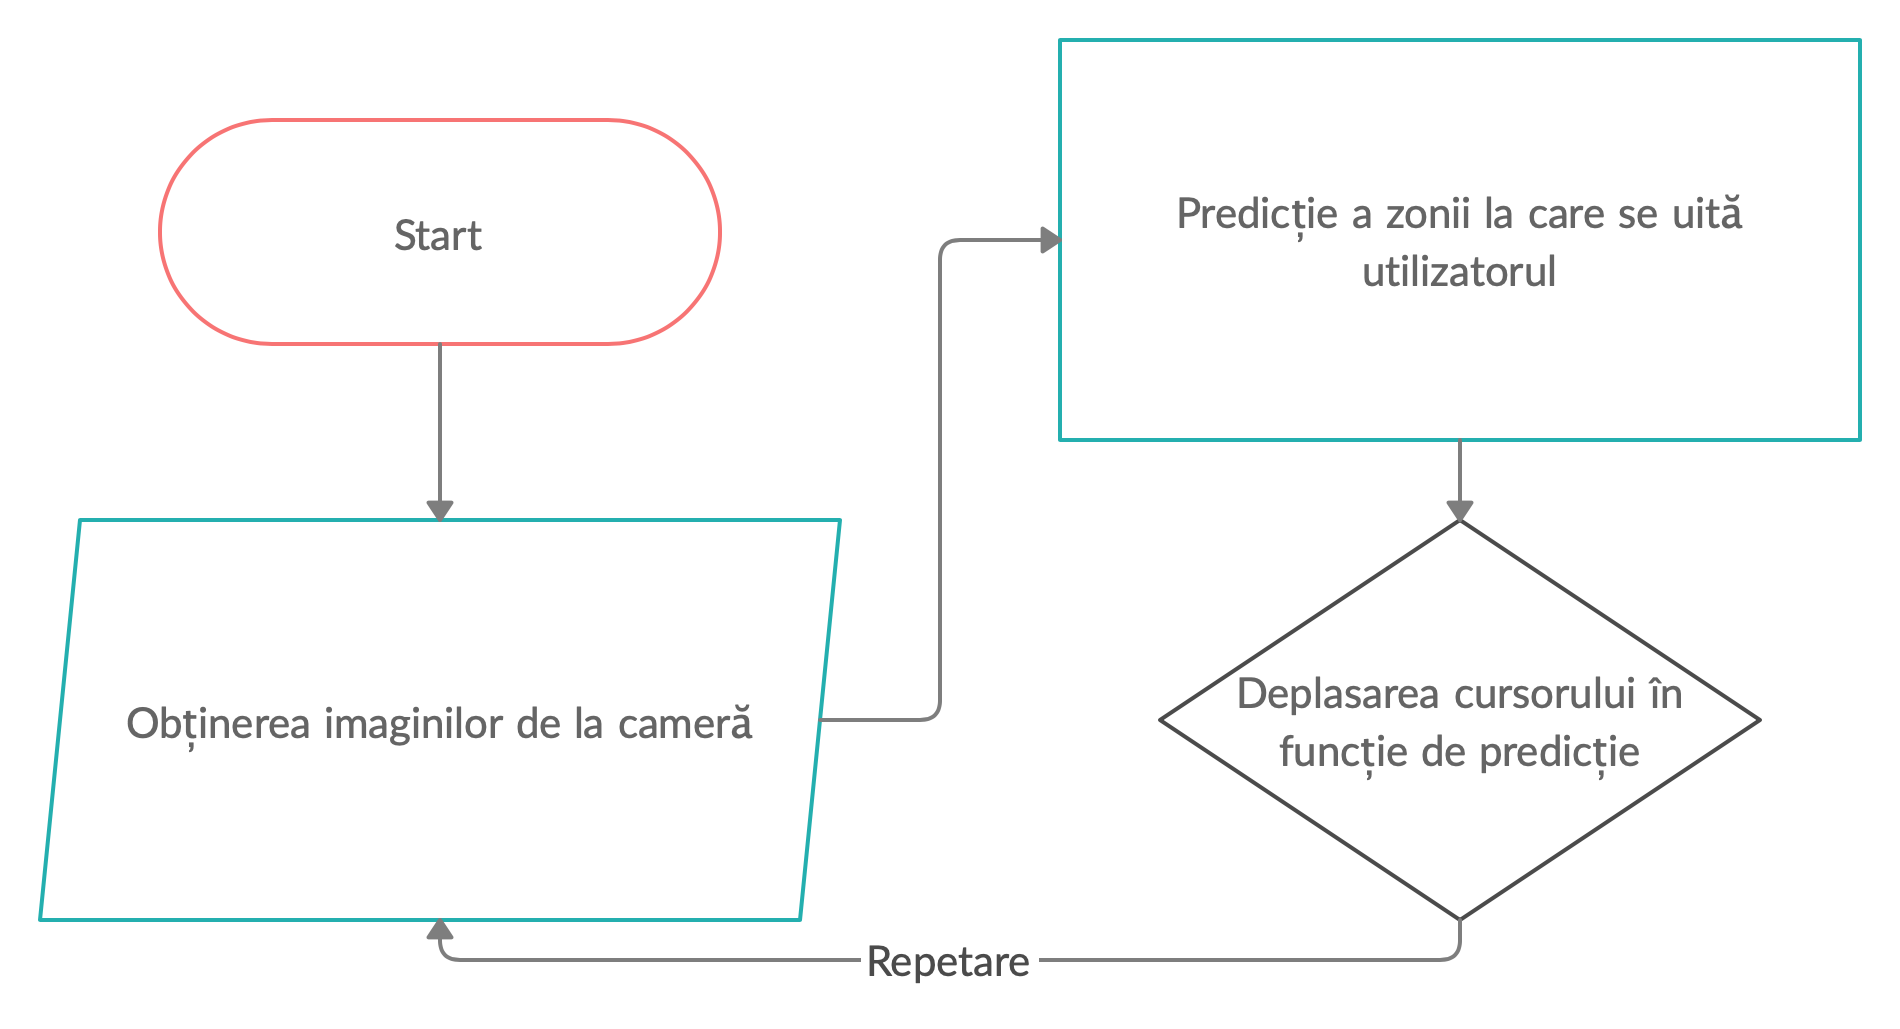
\includegraphics[width=\textwidth]{idee.png}
    \caption{Procedură generală pentru deplasarea mouse-ului}
\end{figure}

\paragraph{}
Această idee nu este nouă și există deja soluții pentru această problemă, bazate pe aceeași idee.
Totuși, cele mai multe dintre ele sunt create ori doar pentru un anumit sistem de operare (în acest caz, Windows), ori nu sunt gratuite și au un cost atașat semnificativ, sau chiar necesită componente hardware adiționale.

\paragraph{}
\emph{Camera Mouse} este o propunere viabilă care urmărește o porțiune fixată a feței (spre exemplu un ochi) și, când acea porțiune își schimbă poziția, se schimbă și poziția cursorului.
Oferă și functionalități de simulare a apăsării pe butoanele mouse-ului, însă funcționează doar pentru sistemele care rulează Windows.
Printre alternative se mai găsesc \emph{IntelliGaze} și produse dezvoltate de \emph{Tobii Dynavox}, dar acestea necesită în primul rând hardware adițional și rulează doar pe Windows.

\section*{Motivație}
\paragraph{}
Când a trebuit să mă decid asupra temei lucrării de licență, am luat în calcul doi factori cheie: viitoarea mea carieră profesională și utilitatea proiectului.
Mi-am dorit să lucrez la un proiect care mi-ar alimenta interesul în Inteligența Artificială și care mi-ar oferi șansa de a aplica cercetarea pe care aș face-o în acest domeniu.
Mai mult, mi-am dorit de asemenea să am și o abordare practică asupra lucrării, astfel încât să construiesc ceva ce ar fi folositor.

\paragraph{}
Cât despre Inteligența Artificială, este inutil să-i subliniem importanța contemporană.
De la aplicabilitatea medicală, conducere/pilotare autonomă, agricultură inteligentă până la frigidere inteligente care-ți spun când ai rămas fără lapte, Inteligența Artificială este larg răspândită și extinderea ei nu se va opri prea curând.
Pentru mine, acesta este un alt motiv pentru a o studia și a o înțelege mai bine, mai ales că o găsim integrată în viața noastră de zi cu zi.

% % As a bonus, I'll have the chance of using some of the knowledge I've gathered as a student throughout the time.
% % to individually work on a project that will showcase my software development skills, but also the abilities of practical knowledge applying and researching on certain topics.

\section*{Obiective}
\paragraph{}
Obiectivul principal al aplicației este acela de a simula funcționalitatea unui mouse.
Așadar, aplicația dezvoltată suportă cele mai importante funcționalități ale acestuia:
\begin{itemize}
    \item mișcarea cursorului
    \item apăsarea butonului stâng\footnote{Această funcționalitate mai este denumită uzual și ``click stânga''}
    \item apăsarea butonului drept\footnote{Această funcționalitate mai este denumită uzual și ``click dreapta''}
\end{itemize}

\paragraph{}
TODO să inserez aici o schema cu mouse

\paragraph{}
În urma analizei produselor deja existente, am vrut să dezvolt o aplicație care constituie un pachet atractiv de beneficii.
Am construit o listă cu obiectivele principale ale aplicației:
\begin{itemize}
    \item să fie cross-platform: aplicația ar trebui să ruleze pe toate sistemele de operare populare: Windows, Linux și MacOS
    \item să țină cont de diferențele fizionomice dintre utilizatori
    \item să aibă o interfață grafică
    \item să fie ușor și intuitiv de folosit
    \item să fie ușor de instalat
\end{itemize}

\paragraph{}
În capitolul 1 va fi prezentată... iar apoi...

\paragraph{}
În restul capitolelor...